\documentclass[a4paper,twocolumn]{article}

\usepackage[english]{babel}
\usepackage[utf8]{inputenc}
\usepackage{graphicx}
\usepackage{fullpage}
\usepackage{amssymb}
\usepackage{caption}

\newenvironment{Figure}
  {\par\medskip\noindent\minipage{\linewidth}}
  {\endminipage\par\medskip}

\title{Progressive Neural Networks $-$ summary}
\author{Matěj Nikl}

\begin{document}
\maketitle
\noindent
Progressive Neural Networks (PNNs) are networks trying to address the task of using, transferring and not forgetting previously learned knowledge to learn yet another task, preferably with faster convergence. It retains a pool of trained models throughout training and learns connections to them to harvest potentially useful features while also learning new ones. What it means is that it has the ability to choose whether the previously learned knowledge is useful for the new task and thus to transfer it, or even to ignore it completely (by zeroing the lateral connections).

    \begin{figure}[!h]
        \centering
        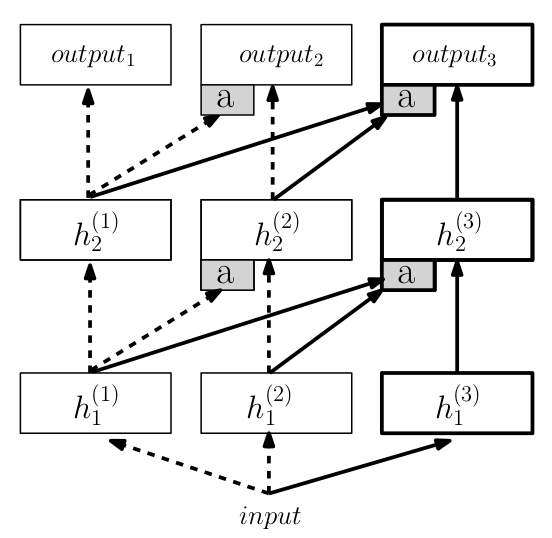
\includegraphics[width=0.75\columnwidth]{PNN.png}
        \caption{A three column progressive network}
    \end{figure}

\subsection*{Basic definition}
A PNN starts with a single column $-$ a DNN with $L$ layers and hidden activations $h_i^{(1)} \in \mathbb{R}^{n_i}$, with $n_i$ the number of units at layer $i \le L$, and parameters $\Theta^{(1)}$ trained to convergence. When adding a second task, the parameters $\Theta^{(1)}$ are ``frozen'' and a new column with parameters $\Theta^{(2)}$ is instantiated (with random initialization), where layer $h_i^{(2)}$ receives input from both $h_{i-1}^{(2)}$ and $h_{i-1}^{(1)}$ via lateral connections. This generalizes to $K$ tasks as follows (biases omitted for clarity):
\[
    h_i^{(k)} = f \left( W_i^{(k)}h_{i-1}^{(k)} + \sum_{j<k} U_i^{(k,j)} h_{i-1}^{(j)} \right)
\]
where $W_i^{(k)} \in \mathbb{R}^{n_i \times n_{i-1}}$ is the weight matrix of layer $i$ of column $k$, $U_i^{(k,j)} \in \mathbb{R}^{n_i \times n_{i-1}}$ are the lateral connections from layer $i-1$ of column $j$, to layer $i$ of column $k$ and $h_0$ is the network input. $f$ is a element-wise non-linearity, $f(x) = \max (0, x)$ for all intermediate layers.

\paragraph{Adapters.} In practice, non-linear lateral connections called \textit{adapters} are used. The serve both to improve initial conditioning and perform dimensionality reduction, so that the number of parameters stemming from the lateral connections is in the same order as $\left| \Theta^{(1)} \right|$ as $k$ grows.

\subsection*{Principles of modularization}
The basic building block of PNNs is a \textit{column}. A column is a neural network with lateral connections to all previously trained columns, each trying to solve just one task. That might encourage the thinking of a column as a potential module. However, it cannot be taken away and used on its own as a some kind of a standalone unit $-$ it always needs all of its previous columns with whom it was trained with to function properly, because it might be extremely dependent on features (knowledge) extracted from input by them. So, even though we might like to see it as a module, it definitely cannot be used that way.


\subsection*{Principles of growing}
For each new task a new column is allocated. The knowledge from all previously learned tasks has the potential to be transferred, while being protected against forgetting, because all previous columns have frozen weights. This way, the PNN can theoretically grow for as many tasks as needed (while potentially transferring the knowledge from all of the previously learned ones), however in practice, some other techniques like pruning and online compression must be used during training for the number of parameters to be reasonable.


    \begin{figure*}[ht]
        \centering
        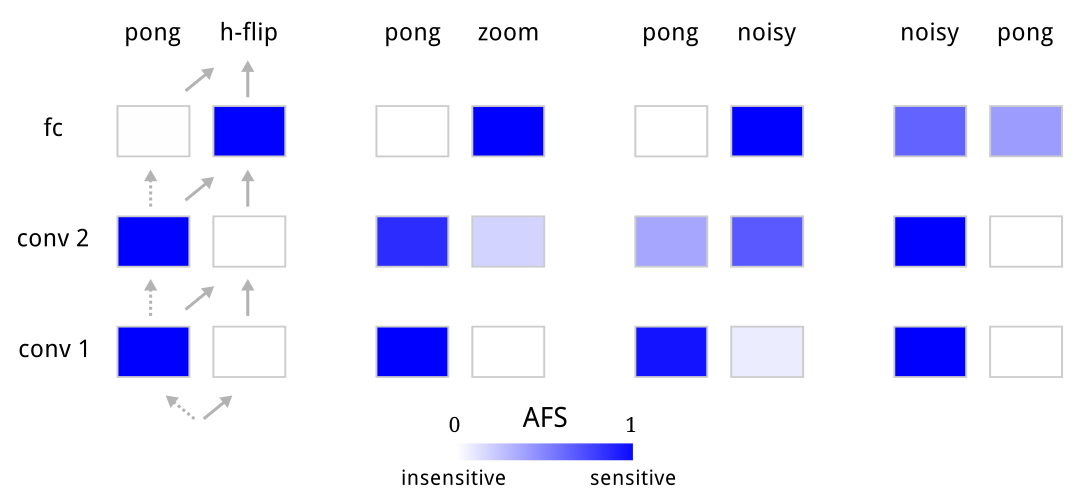
\includegraphics[width=0.65\textwidth]{2-column.png}
        \caption{A two column progressive network $-$ knowledge transfer}
    \end{figure*}

    \begin{figure*}[ht]
        \centering
        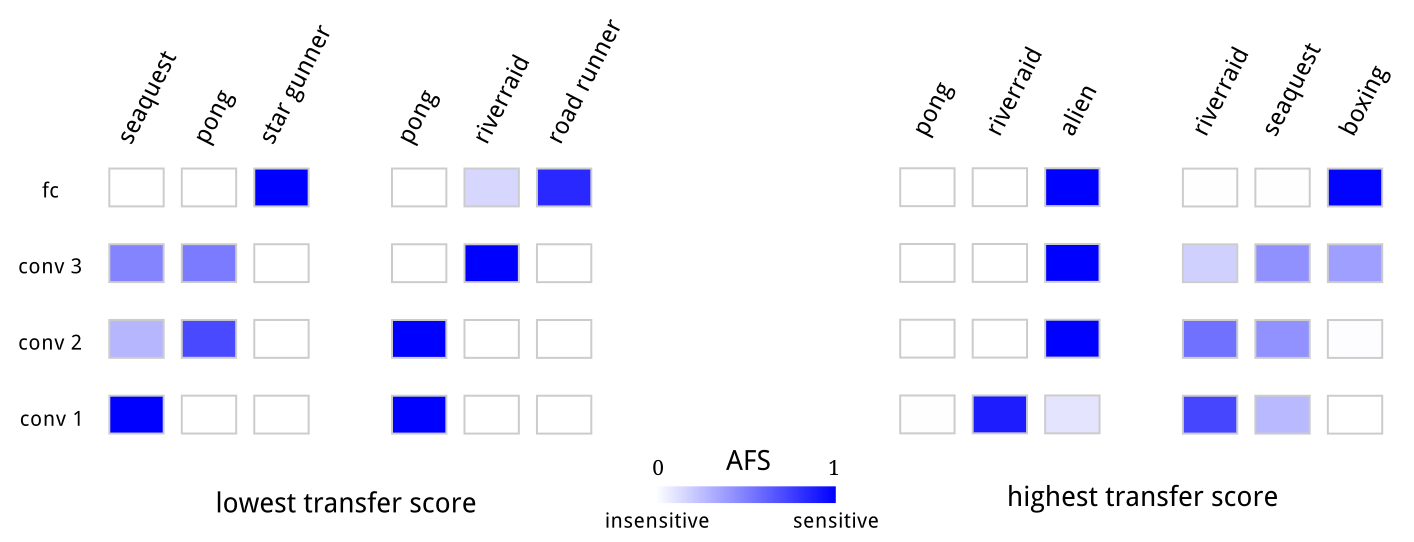
\includegraphics[width=0.9\textwidth]{3-column.png}
        \caption{A three column progressive network $-$ knowledge transfer to the rightmost task}
    \end{figure*}

    \begin{figure*}[ht]
        \centering
        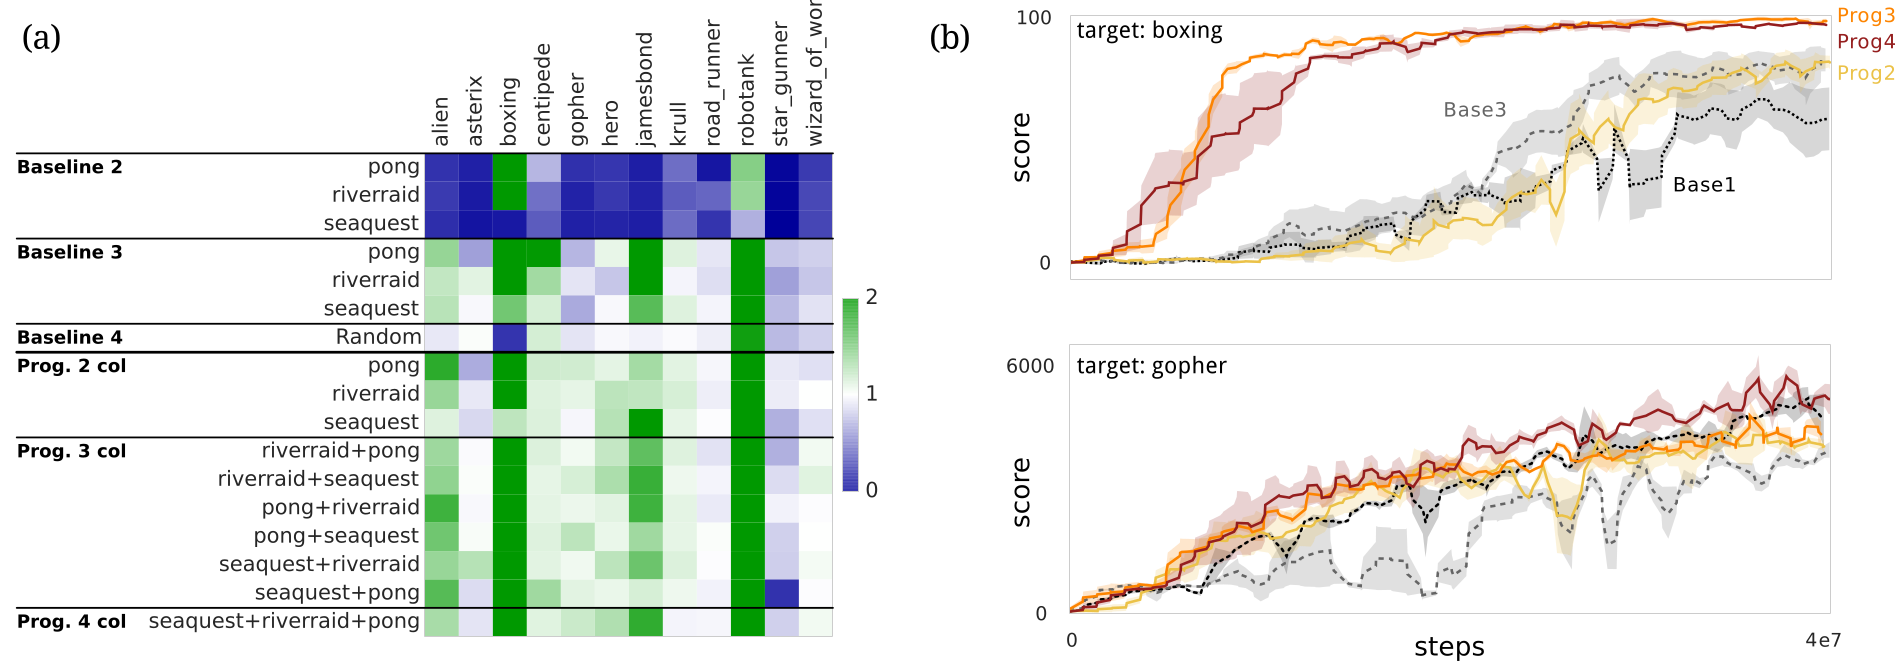
\includegraphics[width=\textwidth]{perf.png}
        \captionsetup{singlelinecheck=off}
        \caption[trololo]{(a) Transfer matrix. Colors indicate transfer scores (clipped at 2). For progressive nets, the first column is trained on Pong, Noisy, or H-flip (table rows); the second column is trained on each of the other pong variants (table columns). (b) Example learning curves. \\
        \begin{itemize}
            \item \textbf{Baseline 2} $-$ a single column, pretrained on a source task and fine-tuned on the target task (output layer only)
            \item \textbf{Baseline 3} $-$ the same as baseline 2 but the whole model is fine-tuned
            \item \textbf{Baseline 4} $-$ a 2 column progressive architecture, with previous columns initialized randomly and frozen
        \end{itemize}
        }
    \end{figure*}

\end{document}
